\chapter{Durchführung}\label{cha:durchfuehrung}
\section{Vorbereitung}\label{sec:vorbereitung}
\subsection{Auswahl der Umgebung und Höhe}\label{sub:auswahlUmgebung}
Für die Durchführung des Experiments müssen verschiedene Vorbereitungen getroffen werden. Zunächst ist der geeignete Ort auszuwählen. Um das Experiment möglichst präzise und unter optimalen Bedingungen durchzuführen, sollte es in einem möglichst dunklen Raum stattfinden. Für diese Arbeit wurde die Dunkelkammer (Zimmer G10) der Kantonsschule am Burggraben bereitgestellt.

Ein weiterer wichtiger Punkt der Vorbereitung betrifft den Untergrund, auf dem das Experiment aufgebaut wird. Im Experimentierkasten sind Verlängerungsstäbe enthalten, die das Experimentieren angenehmer gestalten sollen. Ein Problem dieser Stäbe ist jedoch, dass sie nicht besonders stabil sind, was die Präzision des Experiments beeinträchtigen könnte. Daher wurde in dieser Arbeit die Plattform auf einen Holzklotz gestellt, um das Experiment auf Augenhöhe bei gestrecktem Rücken durchführen zu können. Es ist wichtig, dass die Plattform eben steht, was mit der Wasserwaage auf der Plattform überprüft werden kann. Sollte die Plattform schräg sein, können die verstellbaren Füße genutzt werden, um sie auszubalancieren. Mit diesem Holzklotz wurde der Plattform ein stabiler Untergrund geboten, wodurch das Experiment für die Feinjustierung des optischen Systems vorbereitet war.

\subsection{Kondensatorenabstand messen}\label{sub:kondensatorenabstand}
Der nächste Schritt in der Vorbereitung besteht im Messen des Abstands zwischen den beiden Kondensatoren. Dabei ist es von entscheidender Bedeutung, dass die Spannung während dieses Vorgangs abgeschaltet wird. Zunächst wird das Gehäuse der Betrachtungskammer entfernt. Anschließend wird die obere Platte vorsichtig abgenommen, gefolgt von der Kunststoffplatte darunter.

Im Experimentierkasten befindet sich eine Schieblehre, die zur Messung der Dicke der Kunststoffplatte verwendet wird. Es ist wichtig, dass die Messung am inneren Rand der Platte erfolgt und nicht am äußeren, da der äußere Rand eine leicht größere Dicke aufweist. Der gemessene Wert kann dann direkt abgelesen und dokumentiert werden.

\section{Das optische System ausrichten}\label{sec:optischesSystem}
\subsection{Das Betrachtungsfernrohr fokussieren}
Die Betrachtungskammer sollte nun wieder zusammengebaut werden, wobei das Gehäuse vorerst noch nicht angebracht wird. Der Fokussierdraht auf der Platte ist abzuschrauben und vorsichtig in das Loch in der Mitte der oberen Kondensatorenplatte einzuführen. Anschließend muss die Halogenlampe angeschlossen werden. Dazu wird der Stecker des 12 V DC-Transformators mit der Lampe verbunden, sodass die Lampe zu leuchten beginnt.

Der nächste Schritt besteht darin, das Fadenkreuz in den Fokus zu setzen. Dies erfolgt durch Drehen des Fadenkreuz-Fokussierrings, bis das gesamte Gitter scharf abgebildet wird. Danach ist der Draht durch das Betrachtungsfernrohr zu beobachten und der Tröpfchen-Fokussierring so lange zu drehen, bis der Draht scharf gesehen werden kann.

\subsection{Die Halogenlampe einstellen}\label{sub:Halogenlampe}
Mit dem horizontalen Einstellknopf der Halogenlampe ist das Licht auf der horizontalen Ebene korrekt zu fokussieren. Der optimale Fokus ist erreicht, wenn der rechte Rand des Drahts den höchsten Helligkeitskontrast zur linken Seite aufweist. Mit dem vertikalen Einstellknopf wird das Licht so eingestellt, dass das Zentrum des Gitters bzw. des Fadenkreuzes am hellsten sichtbar ist. Nachdem alle Einstellungen vorgenommen wurden, sollte der Fokussierdraht wieder in die Vertiefung der Platte verschraubt werden.

\section{Funktionen der Steuerung}\label{sec:funktionen}
\subsection{Kondensatorenspannung Schalter}\label{sub:Spannungsschalter}
Dieser Schalter dient als Spannungswechsler für die beiden Kondensatoren und ermöglicht es, die Richtung des elektrischen Feldes $E$ zu ändern. Der Schalter verfügt über drei verschiedene Positionen: Die erste Position, "plates grounded", bedeutet, dass keiner der beiden Kondensatoren geladen ist, wodurch keine elektrische Kraft auf die Tröpfchen wirkt. In der zweiten Position, "TOP PLATE -", ist die obere Platte negativ geladen, wodurch das elektrische Feld nach unten gerichtet ist. Die letzte Position, "TOP PLATE +", bedeutet, dass die obere Platte positiv geladen ist, wodurch das elektrische Feld nach oben zeigt.

\subsection{Der Ionisationsquelle Schalter}\label{sub:ionisationquelle}
Der Schalter für die Ionisation verfügt über drei verschiedene Positionen: die "An"-Position, die "Aus"-Position und die "Tröpfchensprüh"-Position. In der "Aus"-Position wird die Ionisationsquelle vollständig abgeschirmt, sodass keine Alphateilchen in die Kammer gestrahlt werden können. In der "An"-Position ist diese Abschirmung entfernt, sodass die Öltröpfchen ionisiert und angestrahlt werden können. Die "Tröpfchensprüh"-Position wird aktiviert, wenn die Öltröpfchen in die Kammer eingesprüht werden. In dieser Position öffnet sich ein kleines Loch in der Kammer, das den Luftstrom ermöglicht, während das Öl eingesprüht wird.

\begin{figure}[ht]
	\begin{center}
		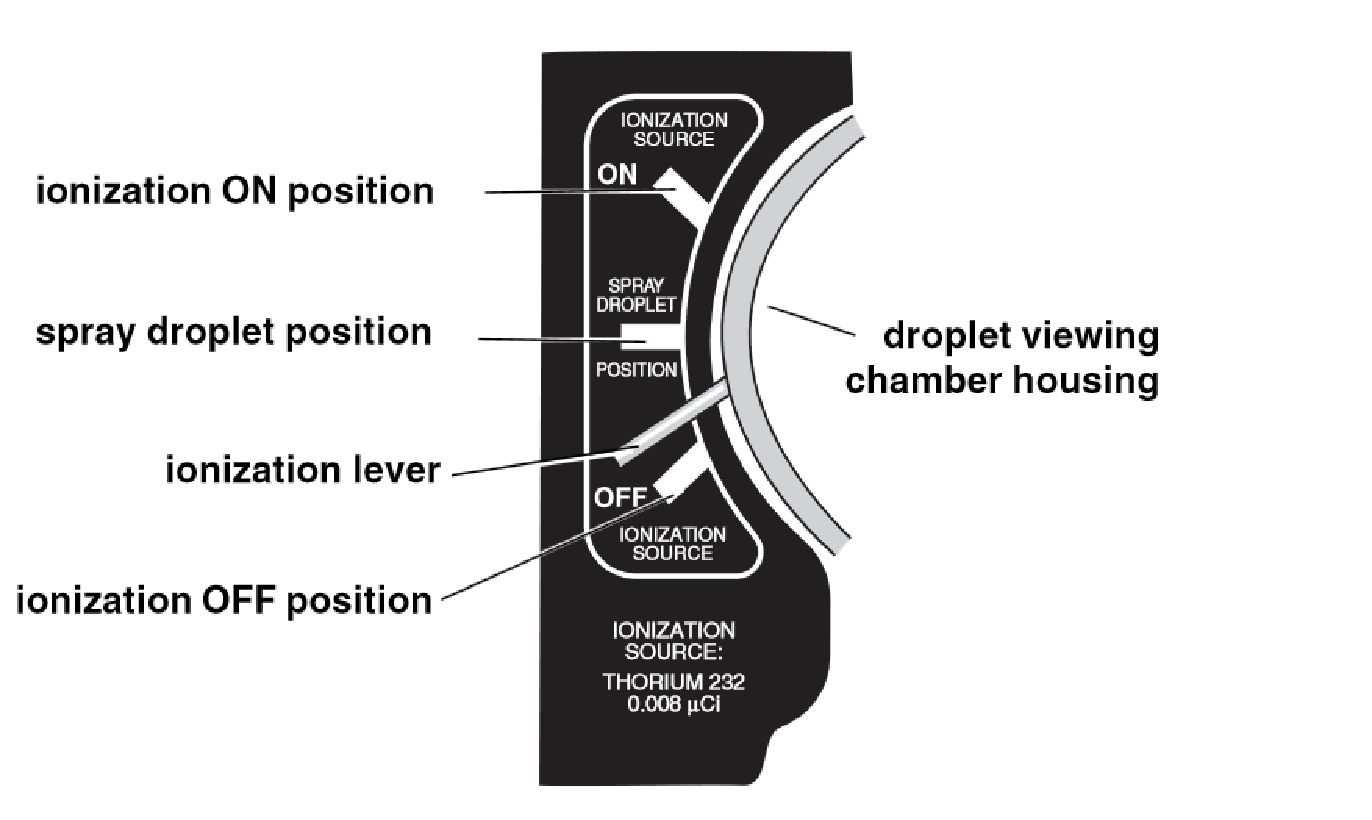
\includegraphics[scale=0.5]{bilder/pdf/Schalterfunktionen.pdf}
		\caption{Schalterpositionen der Ionisationsquelle}
		\label{fig:Schalterpositionen}
	\end{center}
\end{figure}

\section{Messen und Einstellen der Spannung}\label{sec:spannung}
Zunächst muss die Gleichstromquelle über die farbigen Anschlüsse mit der Plattform verbunden werden. Das digitale Multimeter kann parallel zu den Kontakten eingebaut werden. Nach dem Einschalten des Multimeters muss der Modus auf Gleichstromspannung eingestellt werden. Wenn die Stromquelle eingeschaltet wird, sollte das Multimeter eine Spannung von etwa 500 V anzeigen. Falls dies nicht der Fall ist, muss die Spannung an der Stromquelle entsprechend angepasst werden. Es ist wichtig zu betonen, dass aufgrund der in den Kondensatoren eingebauten großen Widerstände keine Gefahr eines elektrischen Schocks besteht.

\section{Temperatur in der Tröpfchenkammer}\label{sec:Temperatur}
Die letzte erforderliche Einstellung, bevor mit dem eigentlichen Experiment begonnen werden kann, besteht darin, die Temperatur innerhalb der Tröpfchenkammer zu messen. Die Temperatur ist notwendig, um die Viskosität der Luft zu bestimmen. Da die genaue Temperatur nicht direkt mit einem Thermometer gemessen werden kann, erfolgt die Bestimmung über die Beziehung zwischen dem elektrischen Widerstand der Kondensatoren und der Temperatur. Der Widerstand wird auf die gleiche Weise wie die Spannung gemessen. Auf der Platte befinden sich Anschlüsse für ein digitales Multimeter, das auf den Messmodus für elektrischen Widerstand eingestellt werden sollte. Der proportionale Zusammenhang zwischen Temperatur und Widerstand kann aus einer Tabelle abgelesen werden. Es ist wichtig, dass die Stromquelle niemals mit den Anschlüssen für den Widerstand verbunden wird, da dies das Experiment beschädigen könnte. Der Widerstand sollte dabei im Bereich von etwa 1 bis 4 Megaohm liegen.

\begin{figure}[ht]
	\begin{center}
		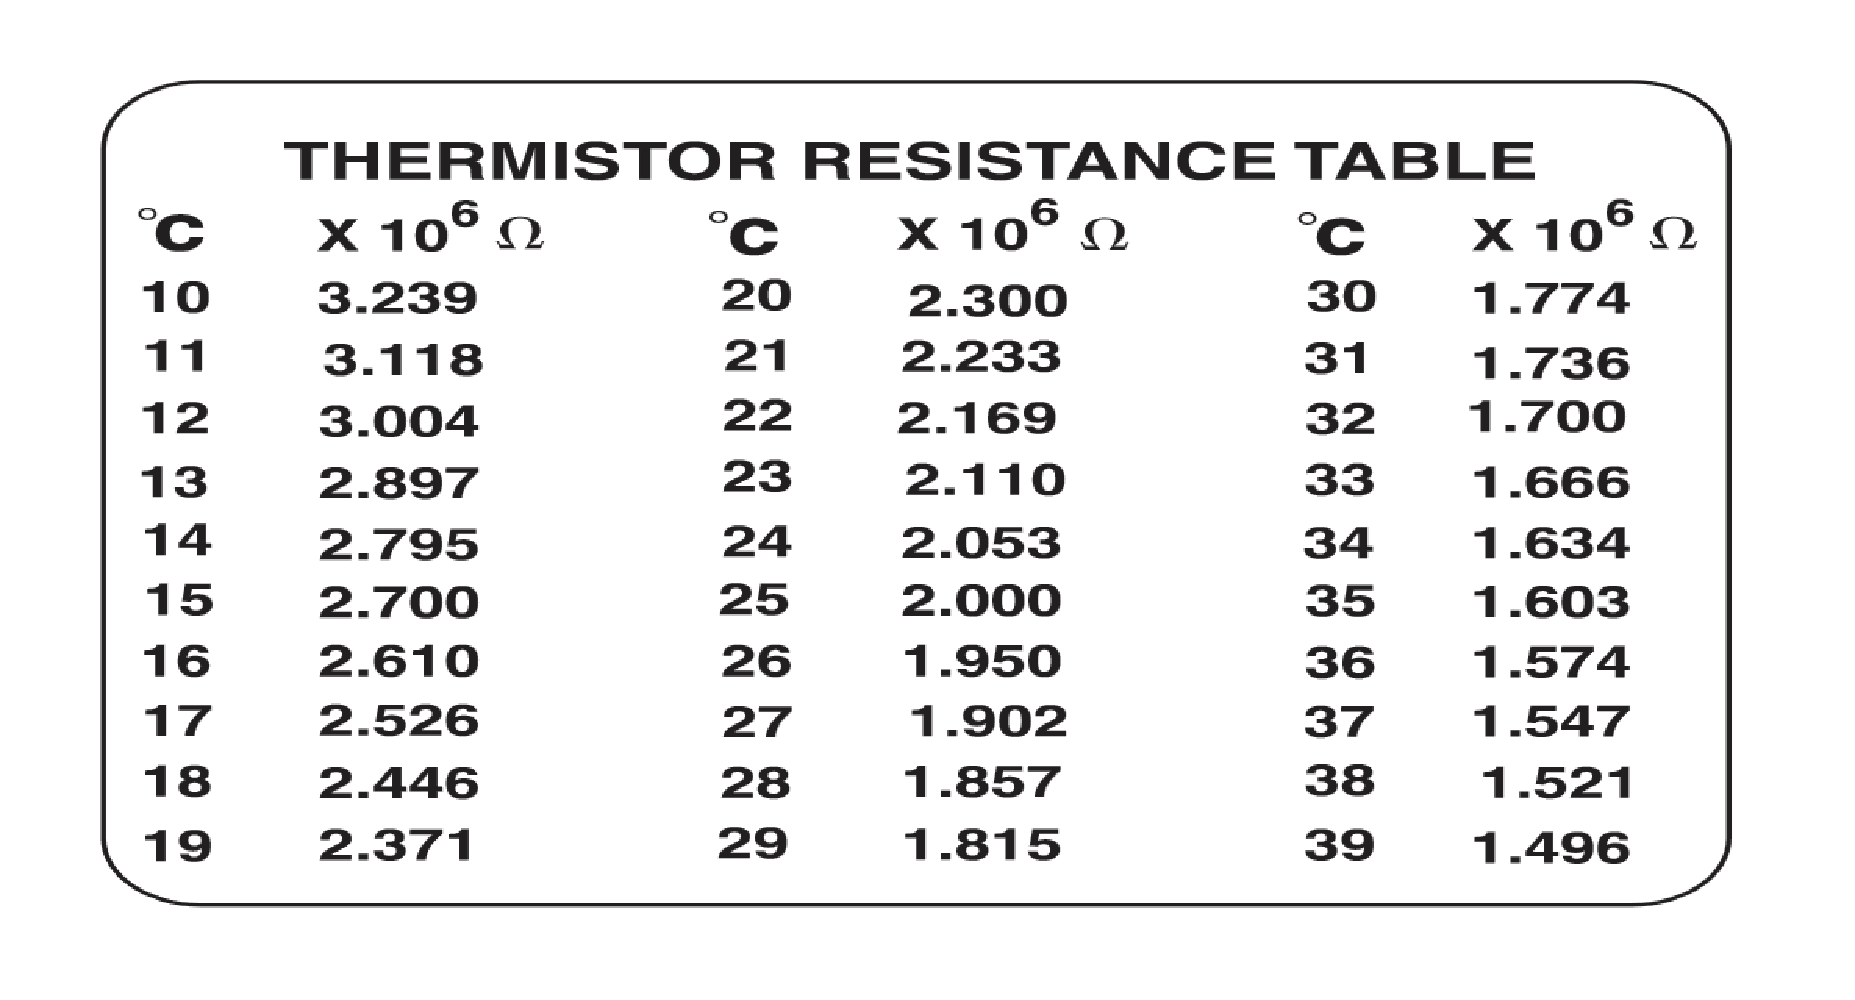
\includegraphics[scale=0.25]{bilder/pdf/TemperaturTabelle.pdf}
		\caption{Abhängigkeit von Temperatur und elektrischer Widerstand}
		\label{fig:widerstandTemperatur}
	\end{center}
\end{figure}

\section{Das Experimentieren}\label{sec:durchfuehrung}
Bevor mit dem Experiment begonnen werden kann, muss die gesamte Kammer wieder zusammengebaut werden. Der Tröpfchenlochschutz sollte auf die Öffnung der oberen Platte montiert werden, um zu verhindern, dass während des Experiments weitere Tröpfchen in die Betrachtungskammer gelangen. Anschließend wird die Spannung sowie die Temperatur erneut kurz überprüft, um sicherzustellen, dass alle Voraussetzungen für den Versuch erfüllt sind, bevor mit dem Experiment fortgefahren wird.

\subsection{Tröpfchen Einsprühen}\label{sub:tröpfchensprühen}
Der erste Schritt besteht in der Vorbereitung des Ölsprühers. Dazu wird Mineralöl, dessen Dichte bekannt ist (z.B. das zugehörige Squibb \#5597 Mineral Oil mit Dichte: $886 kg/m^3$), in den Zerstäuber gefüllt. Anschließend wird versucht, Tröpfchen zu erzeugen, indem mehrfach schnell und mit leichtem Druck auf das Kissen des Zerstäubers gedrückt wird, bis auf einem Papier kleine Tröpfchen sichtbar sind.
\begin{figure}[h]
	\begin{minipage}[t]{0.45\textwidth}
		\centering
		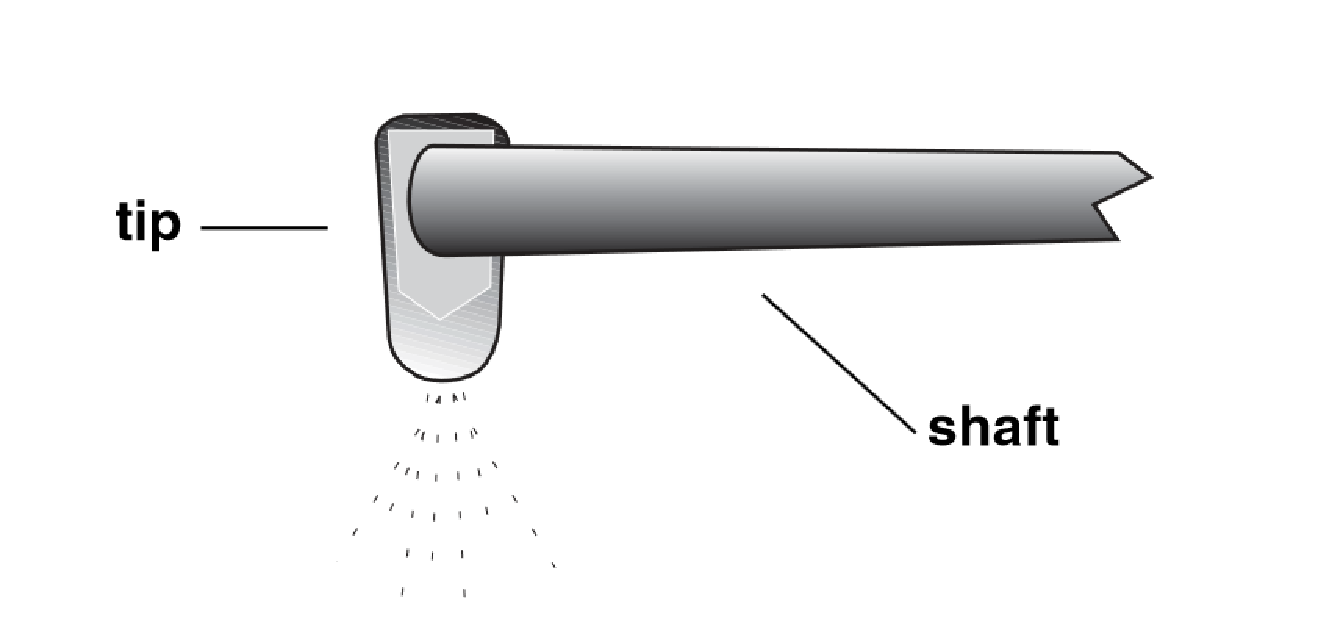
\includegraphics[width=\textwidth]{bilder/pdf/zerstauberSpitze.pdf}
		\caption{Korrekte Position von Spitze zur Achse}
		\label{fig:zerstauberSpitze}
	\end{minipage}
	\hfill
	\begin{minipage}[t]{0.45\textwidth}
		Die Spitze des Zerstäubers muss nach unten schauen. Genau 90° zur Achse. (siehe \autoref{fig:zerstauberSpitze})
	\end{minipage} 
\end{figure}

Nach diesem Schritt muss der Schalter der Ionisationsquelle auf die "Tröpfchensprüh-Position" gestellt werden, um sicherzustellen, dass während des Einsprühens die Luft aus der Kammer entweichen kann. Da die Spitze des Zerstäubers nach unten zeigt, kann dieser nun direkt in das vorgesehene Loch auf dem Deckel des Gehäuses eingeführt werden. Jetzt sollte durch das Betrachtungsfernrohr geschaut werden, während gleichzeitig kräftig auf das Kissen des Zerstäubers gedrückt wird. Anschließend werden mit schwächeren, kleineren Stößen die Tröpfchen ins Sichtfeld des Betrachters gebracht. Sobald eine Ansammlung von kleinen goldenen Punkten sichtbar wird, muss der Schalter auf die "Aus-Position" zurückgesetzt werden.

Das Einsprühen der Tröpfchen stellt zu Beginn eine Herausforderung dar und wird vermutlich nicht beim ersten Versuch erfolgreich sein. Es gibt keine festgelegte Technik für den Umgang mit dem Zerstäuber; der Experimentator muss eine eigene Methode entwickeln, um den Zerstäuber effizient zu bedienen. Dieser Vorgang kann viel Zeit in Anspruch nehmen. In dieser Arbeit stellte sich heraus, dass es am besten funktionierte, den Zerstäuber einmal kräftig zu drücken und danach kleinere, schwächere Stöße zu verabreichen.

Falls zu viele Tröpfchen im Sichtfeld sichtbar sind, empfiehlt es sich, drei bis vier Minuten zu warten, bis die meisten Tröpfchen verschwunden sind. Danach kann das Experiment in Ruhe fortgesetzt werden.

\subsection{Auswahl des richtigen Tröpfchen}\label{sub:auswahlTropfen}
Von den sichtbaren Tröpfchen sollte eines ausgewählt werden, dessen Fallgeschwindigkeit etwa zwischen $0.02$ und $0.05$ mm/s liegt, wenn der Schalter der Kondensatoren auf "plates grounded" gestellt ist. Die Fallgeschwindigkeit sollte so gewählt werden, dass das Tröpfchen sich mit dem Schalter vertikal verstellen lässt. Diese spezifische Beschreibung der Fallgeschwindigkeit ist schwierig genau zu messen. Ein hilfreicher Hinweis: Ein Tröpfchen, das etwa 15 Sekunden benötigt, um die Distanz zwischen zwei Hauptlinien des Gitters ($0.5$ mm) zu durchqueren, bewegt sich mit einer Geschwindigkeit von ungefähr $0.03$ mm/s.

Sollten immer noch zu viele Tröpfchen im Sichtfeld sichtbar sein, kann es hilfreich sein, für kurze Zeit die Kondensatoren zu laden, um die meisten Tröpfchen zu entfernen. Da nicht alle Tröpfchen eine Nettoladung aufweisen und daher nicht beeinflusst werden, kann der Ionisationsschalter für drei bis fünf Sekunden in die "An-Position" geschaltet werden, um sicherzustellen, dass sich alle Tröpfchen bewegen lassen.

Sobald ein geeignetes Tröpfchen gefunden wurde, dessen Fallgeschwindigkeit innerhalb der gewünschten Größenordnung liegt, kann der Fokussierring verwendet werden, um das Tröpfchen weiter zu schärfen. Dies entlastet die Augen des Experimentators und ermöglicht eine längere Beobachtungsdauer. Der beste Fokus ist erreicht, wenn das Tröpfchen wie eine goldene Nadelspitze erscheint.

\subsection{Daten sammeln mit der Fall und Steigzeit}\label{sub:datenFallundSteig}
Zur Bestimmung der Ladung eines Öltröpfchens müssen sowohl die Steiggeschwindigkeit (bei geladenen Kondensatoren) als auch die Sinkgeschwindigkeit (bei nicht geladenen Kondensatoren) gemessen werden. Die genaueste Messung erfolgt, indem die Zeit gemessen wird, die das Tröpfchen benötigt, um von der ersten großen Linie bis zur zweiten großen Linie zu gelangen. Diese Linien sind exakt $0.5$ mm voneinander entfernt. Die Geschwindigkeit $v$ kann dann mit der einfachen Formel $v = \frac{s}{t}$ berechnet werden, wobei $s$ die zurückgelegte Strecke und $t$ die benötigte Zeit ist. Ein Beispiel: Wenn ein Tröpfchen $15$ Sekunden benötigt, um die Strecke von $0.5$ mm zu überwinden, ergibt sich die Geschwindigkeit zu $v = \frac{0.5,\text{mm}}{15,\text{s}} = 0.033,\text{mm/s} = 3.3 \cdot 10^{-5},\text{m/s}$.

Für präzisere Ergebnisse sollte die Geschwindigkeit eines Tröpfchens etwa 5 bis 15 Mal gemessen werden.

Nach der ersten Messung kann die Ladung des Tröpfchens provisorisch geschätzt werden. Falls die gemessene Ladung mehr als das Fünffache der Elementarladung beträgt, sollte für die weiteren Messungen ein langsameres Tröpfchen gewählt werden.

Anschließend sollten neue Tröpfchen eingesprüht und die Geschwindigkeiten erneut gemessen werden, bis das Tröpfchen seine Ladung spontan ändert oder aus dem Sichtfeld verschwindet. Die Ladung eines Tröpfchens kann durch den Ionisationsschalter verändert werden. In diesem Schritt sollten die Messungen so oft wie möglich wiederholt werden, um eine möglichst präzise Bestimmung der Ladung zu erhalten. Sollte die Beobachtung durch Ermüdung beeinträchtigt werden, können alternative Messgrößen wie die Spannung, die Zähigkeit der Luft, die Dichte des Öls und der Luftdruck aufgezeichnet werden. Alle Messdaten sollten in einer Tabelle dokumentiert werden, bevor mit der Berechnung der Ladungen aus den einzelnen Messungen fortgefahren wird.

\subsection{Methode für die Berechnung der Ladung}\label{sub:methodeBerechnung}
Mit der Formel in \autoref{eq:qRadius} kann zuerst der Radius $a$ berechnet werden:
\begin{equation*}
	a \ = \ \sqrt{\left( \frac{b}{2p}\right)^2 + \frac{9\eta v_f}{2\rho g}} - \frac{b}{2p}
\end{equation*}

\noindent Dann kann die Masse $m$ des Tröpfchens berechnet werden indem man die Formel für den Radius in die Formel für die Masse Substituiert:
\begin{equation*}
	\begin{split}
		m & \ = \ \frac{4}{3}\pi a^3 \rho \\
		& \ = \ \frac{4}{3}\pi \left( \sqrt{\left( \frac{b}{2p}\right)^2 + \frac{9\eta v_f}{2\rho g}} - \frac{b}{2p} \right)^3 \rho
	\end{split}
\end{equation*}

\noindent Der letzte Schritt ist die Masse $m$ in der \autoref{eq:hauptgleichung} zu substituieren:
\begin{equation*}
	\begin{split}
		q & \ = \ \frac{m g (v_f + v_r)}{Ev_f} \\
		& \ = \ \frac{4}{3} \pi \rho g \left( \sqrt{\left( \frac{b}{2p}\right)^2 + \frac{9\eta v_f}{2\rho g}} - \frac{b}{2p} \right)^3 \frac{(v_f + v_r)}{Ev_f}
	\end{split}
\end{equation*}

\noindent Wenn man das $E$ jetzt noch mit der \autoref{eq:elektrischeFeldstärke} ersetzt hat man die Ladung $q$ eines Tröpfchens:
\begin{equation*}
	q_{tröpfchen} \ = \ \frac{4}{3} \pi \rho g \left( \sqrt{\left( \frac{b}{2p}\right)^2 + \frac{9\eta v_f}{2\rho g}} - \frac{b}{2p} \right)^3 \frac{d(v_f + v_r)}{Vv_f}
\end{equation*}







